\documentclass[11pt]{article}
\usepackage[margin=1in]{geometry}
\usepackage[T1]{fontenc}
\usepackage[utf8]{inputenc}
\usepackage{lmodern}
\usepackage{setspace}
\usepackage{booktabs}
\usepackage{longtable}
\usepackage{array}
\usepackage{amsmath}
\usepackage{amssymb}
\usepackage{hyperref}
\usepackage{xcolor}
\usepackage{tikz}
\usetikzlibrary{arrows.meta, positioning, shapes.geometric, fit, calc}

\hypersetup{
    colorlinks=true,
    linkcolor=blue,
    urlcolor=blue,
    citecolor=blue
}

\setlength{\parskip}{0.5em}
\setlength{\parindent}{0pt}
\onehalfspacing

\title{%
Clock--Phase--Motor Architecture with IMU-Driven PPO\\
for Hexapod Gait Parameter Tuning\\[0.5em]
\large ODE-Based Simulation and Reinforcement Learning Design Document
}
\author{E90 Hexapod Team}
\date{\today}

\begin{document}
\maketitle
\tableofcontents
\newpage

%% ===================================================================
\section{Introduction and Motivation}
%% ===================================================================

This document presents the detailed design for a \textbf{lightweight, ODE-based hexapod gait simulator} integrated with \textbf{Proximal Policy Optimization (PPO)} to tune gait architecture parameters using \textbf{IMU feedback}. The system is intended to fill the currently empty \texttt{ode\_optimization\_with\_imu/} folder and extend the existing open-loop no-IMU optimizer into a closed-loop learning system.

\subsection{Why This Step Matters}

The project roadmap defines a progression from open-loop gait optimization to closed-loop adaptive control:

\begin{enumerate}
    \item \textbf{No-IMU ODE optimization} (completed): SciPy SLSQP tunes 25 gait parameters against a reduced body ODE. The optimizer minimizes roll/pitch RMS, frequency tracking error, and servo overuse. There is no feedback during the simulated gait---parameters are fixed for each trial.
    \item \textbf{IMU-driven ODE optimization with PPO} (this document): The gait runs in a body ODE that produces IMU-like signals (roll, pitch, angular rates). A PPO agent observes these signals at each gait window and adjusts a compact set of architecture parameters (reflex gains, stride/height/frequency scaling). The agent learns \emph{when} and \emph{how much} to adjust parameters in response to body state.
    \item \textbf{Full MuJoCo PPO} (future): Transfer lessons from the lightweight ODE+PPO to the full rigid-body MuJoCo hexapod environment already implemented in \texttt{e90\_repo/}.
    \item \textbf{Hardware deployment} (future): Export the trained parameter-tuning policy to Teensy firmware, receiving real BNO055 IMU data.
\end{enumerate}

The lightweight ODE simulator is fast (approximately 5\,ms per gait cycle on a single CPU core), enabling rapid PPO iteration without the overhead of MuJoCo. This makes it the ideal testbed for validating the clock--phase--motor--PPO architecture before committing to heavier simulation or hardware.

\subsection{Scope of This Document}

This report covers:
\begin{itemize}
    \item The clock--phase--motor architecture and its mathematical formulation
    \item The extended body ODE with IMU signal extraction and reflex coupling
    \item The Gymnasium environment wrapping the ODE as an RL problem
    \item PPO formulation: observation space, action space, reward function, and hyperparameters
    \item Feasibility analysis and risk assessment
    \item Implementation plan with file-by-file specification
    \item Relationship to existing codebase components
\end{itemize}

%% ===================================================================
\section{System Architecture}
\label{sec:architecture}
%% ===================================================================

\subsection{High-Level Data Flow}

The system has five interconnected layers. At each reinforcement learning step, data flows as follows:

\begin{center}
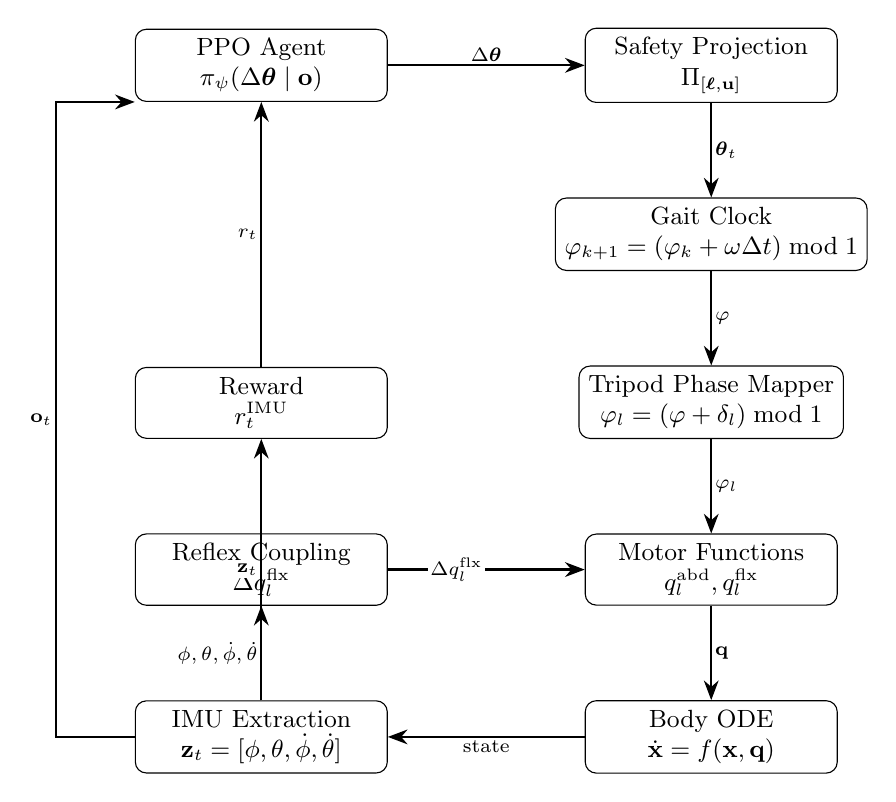
\begin{tikzpicture}[
    node distance=1.2cm and 2.2cm,
    block/.style={rectangle, draw, rounded corners, minimum width=3.2cm, minimum height=0.9cm, align=center, font=\small},
    arrow/.style={-{Stealth[length=2.5mm]}, thick},
    label/.style={font=\scriptsize, midway, fill=white, inner sep=1pt},
]

\node[block] (ppo)   {PPO Agent\\$\pi_\psi(\Delta\boldsymbol{\theta}\mid\mathbf{o})$};
\node[block, right=2.5cm of ppo] (proj)  {Safety Projection\\$\Pi_{[\boldsymbol{\ell},\mathbf{u}]}$};
\node[block, below=of proj] (clock) {Gait Clock\\$\varphi_{k+1}=(\varphi_k+\omega\Delta t)\bmod 1$};
\node[block, below=of clock] (phase) {Tripod Phase Mapper\\$\varphi_l=(\varphi+\delta_l)\bmod 1$};
\node[block, below=of phase] (motor) {Motor Functions\\$q_l^{\mathrm{abd}},q_l^{\mathrm{flx}}$};
\node[block, left=2.5cm of motor] (reflex) {Reflex Coupling\\$\Delta q_l^{\mathrm{flx}}$};
\node[block, below=of motor] (ode)   {Body ODE\\$\dot{\mathbf{x}}=f(\mathbf{x},\mathbf{q})$};
\node[block, left=2.5cm of ode]   (imu)   {IMU Extraction\\$\mathbf{z}_t=[\phi,\theta,\dot\phi,\dot\theta]$};
\node[block, above=of reflex]  (reward) {Reward\\$r_t^{\mathrm{IMU}}$};

\draw[arrow] (ppo)    -- node[label,above]{$\Delta\boldsymbol{\theta}$} (proj);
\draw[arrow] (proj)   -- node[label,right]{$\boldsymbol{\theta}_t$} (clock);
\draw[arrow] (clock)  -- node[label,right]{$\varphi$} (phase);
\draw[arrow] (phase)  -- node[label,right]{$\varphi_l$} (motor);
\draw[arrow] (motor)  -- node[label,right]{$\mathbf{q}$} (ode);
\draw[arrow] (ode)    -- node[label,below]{state} (imu);
\draw[arrow] (imu)    -- node[label,left]{$\phi,\theta,\dot\phi,\dot\theta$} (reflex);
\draw[arrow] (reflex) -- node[label,left]{$\Delta q_l^{\mathrm{flx}}$} (motor);
\draw[arrow] (imu)    -- node[label,left]{$\mathbf{z}_t$} (reward);
\draw[arrow] (reward) -- node[label,left]{$r_t$} (ppo);
\draw[arrow] (imu.west) -- ++(-1.0,0) |- node[label, near start, left]{$\mathbf{o}_t$} (ppo.south west);

\end{tikzpicture}
\end{center}

\subsection{Layer Descriptions}

\begin{description}
    \item[PPO Agent:] A Stable-Baselines3 PPO policy network. Observes IMU state and gait clock phase. Outputs bounded parameter deltas $\Delta\boldsymbol{\theta}\in\mathbb{R}^7$.
    \item[Safety Projection:] Applies box constraints and slew-rate limits to ensure parameters remain in the safe operating region: $\boldsymbol{\theta}_{t+1}=\Pi_{[\boldsymbol{\ell},\mathbf{u}]}(\boldsymbol{\theta}_t+\Delta\boldsymbol{\theta}_t)$.
    \item[Gait Clock:] A phase oscillator $\varphi\in[0,1)$ advancing at angular frequency $\omega=s_{\mathrm{freq}}\cdot\omega_0$. This is the single timing source for the entire gait.
    \item[Tripod Phase Mapper:] Splits the global clock into per-leg local phases with tripod offsets: $\delta_l=0$ for Tripod~A (FL, MR, RL) and $\delta_l=0.5$ for Tripod~B (FR, ML, RR).
    \item[Motor Functions:] Maps each leg's local phase to abduction and flexion servo commands using sinusoidal waveforms with per-leg rest angles, amplitudes, and phase shifts.
    \item[Reflex Coupling:] IMU-derived roll and pitch corrections are distributed to each leg's flexion command based on the leg's side ($s_l$) and front-rear position ($r_l$).
    \item[Body ODE:] An 8-state reduced body model solved with \texttt{scipy.integrate.solve\_ivp}. States: $[x, \dot{x}, z, \dot{z}, \phi, \dot{\phi}, \theta, \dot{\theta}]$ (longitudinal position, vertical height, roll, pitch).
    \item[IMU Extraction:] Reads roll $\phi$, pitch $\theta$, and their rates $\dot\phi,\dot\theta$ from the ODE state. Computes angular accelerations $\ddot\phi,\ddot\theta$ via finite differences. These are the signals a real BNO055 IMU would provide.
    \item[Reward:] Evaluates gait quality from IMU signals using an exponential stability metric plus forward velocity bonus and effort penalty.
\end{description}

%% ===================================================================
\section{Clock--Phase--Motor Formulation}
\label{sec:clock-phase-motor}
%% ===================================================================

\subsection{Gait Clock}

Define a normalized global gait phase $\varphi\in[0,1)$ that advances each simulation tick by:
\begin{equation}
\varphi_{k+1} = \bigl(\varphi_k + \omega_k\,\Delta t\bigr) \bmod 1
\label{eq:clock}
\end{equation}
where $\omega_k = s_{\mathrm{freq}} \cdot \omega_0$ is the instantaneous gait frequency (Hz), $s_{\mathrm{freq}}$ is a PPO-tunable frequency scaling factor, and $\omega_0$ is the baseline frequency from the no-IMU optimization (approximately $1.8$\,Hz).

\subsection{Tripod Phase Mapping}

The hexapod has six legs partitioned into two tripod groups:
\begin{align}
\mathcal{A} &= \{\mathrm{FL}, \mathrm{MR}, \mathrm{RL}\} \quad\text{(Tripod A)} \\
\mathcal{B} &= \{\mathrm{FR}, \mathrm{ML}, \mathrm{RR}\} \quad\text{(Tripod B)}
\end{align}

Per-leg local phase with anti-phase coupling:
\begin{equation}
\varphi_l = (\varphi + \delta_l) \bmod 1, \quad
\delta_l =
\begin{cases}
0.0 & l \in \mathcal{A} \\
0.5 & l \in \mathcal{B}
\end{cases}
\label{eq:phase-map}
\end{equation}

This ensures that when Tripod~A legs are in swing phase ($\varphi_l \approx 0.25$), Tripod~B legs are in stance/push phase ($\varphi_l \approx 0.75$), and vice versa.

\subsection{Sinusoidal Motor Functions}

For each leg $l$ (indexed $i=0,\ldots,5$ matching \texttt{LEG\_ORDER = [FL, FR, ML, MR, RL, RR]}), the servo commands are sinusoidal functions of the local phase:
\begin{align}
q_l^{\mathrm{abd}}(t) &= \beta_l^{\mathrm{abd}} + s_{\mathrm{stride}} \cdot A_l^{\mathrm{abd}} \cdot \sin\!\bigl(2\pi\varphi_l + \psi_l^{\mathrm{abd}}\bigr) \label{eq:abd-cmd} \\
q_l^{\mathrm{flx}}(t) &= \beta_l^{\mathrm{flx}} + s_{\mathrm{height}} \cdot A_l^{\mathrm{flx}} \cdot \sin\!\bigl(2\pi\varphi_l + \psi_l^{\mathrm{flx}}\bigr) \label{eq:flx-cmd}
\end{align}
where:
\begin{itemize}
    \item $\beta_l^{\mathrm{abd}}, \beta_l^{\mathrm{flx}}$: per-leg rest angles (radians), from no-IMU optimization
    \item $A_l^{\mathrm{abd}}, A_l^{\mathrm{flx}}$: per-leg amplitudes (radians), from no-IMU optimization defaults
    \item $\psi_l^{\mathrm{abd}}, \psi_l^{\mathrm{flx}}$: per-leg phase shifts (radians), from no-IMU optimization
    \item $s_{\mathrm{stride}}$: stride amplitude scale (PPO-tunable, dimensionless)
    \item $s_{\mathrm{height}}$: lift height scale (PPO-tunable, dimensionless)
\end{itemize}

The tripod phase offset $\delta_l$ is already embedded in $\varphi_l$ via Equation~\eqref{eq:phase-map}, plus the existing per-servo phase shifts from the original no-IMU TRIPOD\_PHASE dictionary ($0$ for Tripod~A, $\pi$ for Tripod~B) ensure anti-phase coupling.

\subsection{Reflex Coupling}
\label{sec:reflex}

IMU measurements of roll $\phi$ and pitch $\theta$ are fed back to each leg's flexion command. Define:
\begin{align}
\Delta_{\mathrm{roll}} &= K_\phi\,\phi + K_{\dot\phi}\,\dot\phi \label{eq:reflex-roll} \\
\Delta_{\mathrm{pitch}} &= K_\theta\,\theta + K_{\dot\theta}\,\dot\theta \label{eq:reflex-pitch}
\end{align}
where $K_\phi, K_{\dot\phi}, K_\theta, K_{\dot\theta}$ are reflex gains (PPO-tunable).

Per-leg flexion correction:
\begin{equation}
\Delta q_l^{\mathrm{flx}} = s_l \cdot \Delta_{\mathrm{roll}} + r_l \cdot \Delta_{\mathrm{pitch}}
\label{eq:reflex-per-leg}
\end{equation}
with coupling signs:

\begin{center}
\begin{tabular}{lcccccc}
\toprule
& FL & FR & ML & MR & RL & RR \\
\midrule
Side sign $s_l$ & $+1$ & $-1$ & $+1$ & $-1$ & $+1$ & $-1$ \\
Front-rear sign $r_l$ & $-1$ & $-1$ & $0$ & $0$ & $+1$ & $+1$ \\
\bottomrule
\end{tabular}
\end{center}

\textbf{Physical interpretation:}
\begin{itemize}
    \item $s_l$: when the body rolls left ($\phi>0$), left legs extend (push down) and right legs retract to level the body.
    \item $r_l$: when the body pitches nose-down ($\theta>0$), rear legs extend and front legs retract to level the body. Middle legs are unaffected by pitch correction.
\end{itemize}

Final flexion command with reflex:
\begin{equation}
\hat{q}_l^{\mathrm{flx}} = q_l^{\mathrm{flx}} + \Delta q_l^{\mathrm{flx}}
\label{eq:final-flx}
\end{equation}

%% ===================================================================
\section{Body ODE with IMU Signals}
\label{sec:body-ode}
%% ===================================================================

\subsection{State Vector}

The reduced body model tracks eight state variables:
\begin{equation}
\mathbf{x} = [x,\ \dot{x},\ z,\ \dot{z},\ \phi,\ \dot\phi,\ \theta,\ \dot\theta]^\top
\label{eq:state}
\end{equation}
where $x$ is longitudinal (forward) position, $z$ is vertical (height), $\phi$ is roll angle, and $\theta$ is pitch angle. All positions are in meters and angles in radians.

\subsection{Equations of Motion}

The body ODE computes forces from leg contact and thrust:

\begin{align}
\ddot{x} &= \frac{F_{\mathrm{thrust}} - c_x\,\dot{x}}{m} \label{eq:x-ddot} \\
\ddot{z} &= \frac{F_{\mathrm{vertical}} - m\,g - c_z\,\dot{z}}{m} \label{eq:z-ddot} \\
\ddot{\phi} &= \frac{\tau_{\mathrm{roll}}}{I_\phi} \label{eq:roll-ddot} \\
\ddot{\theta} &= \frac{\tau_{\mathrm{pitch}}}{I_\theta} \label{eq:pitch-ddot}
\end{align}

where:
\begin{itemize}
    \item $m$: total robot mass (chassis + battery + 12 servos $\approx 0.46$\,kg)
    \item $g = 9.81$\,m/s$^2$: gravitational acceleration
    \item $c_x, c_z$: longitudinal and vertical damping coefficients
    \item $I_\phi, I_\theta$: roll and pitch moments of inertia
\end{itemize}

\subsubsection{Contact Model}

Foot contact is modeled as a smooth sigmoid function of flexion angle:
\begin{equation}
w_l = \frac{1}{1 + \exp\!\bigl(-\kappa\cdot(\hat{q}_l^{\mathrm{flx}} - \beta_l^{\mathrm{flx}})/A_l^{\mathrm{flx}}\bigr)}
\label{eq:contact}
\end{equation}
where $\kappa$ is contact sharpness (from \texttt{RobotSpec.contact\_sharpness} $\approx 5.5$). When the leg is flexed below rest, $w_l\to 0$ (lifted); when extended, $w_l\to 1$ (in contact).

\subsubsection{Vertical Forces}

Per-leg vertical force:
\begin{equation}
F_l^z = w_l \cdot \left(\frac{mg}{N_{\mathrm{active}}} + k_s(\hat{q}_l^{\mathrm{flx}} - \beta_l^{\mathrm{flx}}) - \frac{c_s}{N_{\mathrm{active}}}\dot{z}\right)
\label{eq:vert-force}
\end{equation}
where $k_s$ is support gain, $c_s$ is support damping, and $N_{\mathrm{active}}=\max(\sum_l w_l, 1)$.

\subsubsection{Thrust Forces}

Forward thrust from abduction velocity:
\begin{equation}
F_l^x = -w_l \cdot k_{\mathrm{stride}} \cdot \dot{q}_l^{\mathrm{abd}}
\label{eq:thrust}
\end{equation}

\subsubsection{Roll and Pitch Torques}

\begin{align}
\tau_{\mathrm{roll}} &= \sum_l y_l \cdot F_l^z - c_\phi\,\dot\phi \label{eq:roll-torque} \\
\tau_{\mathrm{pitch}} &= \sum_l x_l \cdot F_l^z - c_\theta\,\dot\theta \label{eq:pitch-torque}
\end{align}
where $x_l, y_l$ are the body-frame coordinates of each leg's hip attachment point.

\subsection{IMU Signal Extraction}

From the ODE state at each integration step, the IMU signal vector is:
\begin{equation}
\mathbf{z}_k = [\phi_k,\ \theta_k,\ \dot\phi_k,\ \dot\theta_k,\ \ddot\phi_k,\ \ddot\theta_k]^\top
\label{eq:imu-vector}
\end{equation}
where $\ddot\phi_k$ and $\ddot\theta_k$ are obtained from the ODE right-hand side (Equations~\eqref{eq:roll-ddot}--\eqref{eq:pitch-ddot}) or by finite differences of $\dot\phi, \dot\theta$.

This matches what a real BNO055 IMU mounted on the hexapod torso would provide:
\begin{center}
\begin{tabular}{lll}
\toprule
\textbf{ODE state} & \textbf{BNO055 output} & \textbf{Noise model} \\
\midrule
$\phi, \theta$ & Euler angles (fusion mode) & $\sigma_{\mathrm{euler}} \approx 1^\circ$ \\
$\dot\phi, \dot\theta$ & Gyroscope X/Y & $\sigma_{\mathrm{gyro}} \approx 0.01$\,rad/s \\
$\ddot\phi, \ddot\theta$ & Finite diff of gyro & Amplifies noise \\
\bottomrule
\end{tabular}
\end{center}

\subsection{Domain Randomization}

To reduce overfitting to the simplified ODE model and improve sim-to-real transfer, the following parameters are randomized at each episode reset:

\begin{center}
\begin{tabular}{lccc}
\toprule
\textbf{Parameter} & \textbf{Nominal} & \textbf{Range} & \textbf{Distribution} \\
\midrule
Total mass $m$ (kg) & 0.458 & $[0.39, 0.53]$ & Uniform \\
Contact sharpness $\kappa$ & 5.5 & $[4.0, 7.0]$ & Uniform \\
Support gain $k_s$ (N/rad) & 32.0 & $[24.0, 40.0]$ & Uniform \\
Support damping $c_s$ (N/(m/s)) & 7.5 & $[5.0, 10.0]$ & Uniform \\
Roll damping $c_\phi$ & 0.06 & $[0.04, 0.08]$ & Uniform \\
Pitch damping $c_\theta$ & 0.07 & $[0.05, 0.09]$ & Uniform \\
IMU noise $\sigma_\phi, \sigma_\theta$ (rad) & 0.0 & $[0, 0.02]$ & Uniform \\
IMU noise $\sigma_{\dot\phi}, \sigma_{\dot\theta}$ (rad/s) & 0.0 & $[0, 0.015]$ & Uniform \\
Initial roll perturbation (rad) & 0.0 & $[-0.05, 0.05]$ & Uniform \\
Initial pitch perturbation (rad) & 0.0 & $[-0.05, 0.05]$ & Uniform \\
\bottomrule
\end{tabular}
\end{center}

%% ===================================================================
\section{PPO Reinforcement Learning Formulation}
\label{sec:ppo}
%% ===================================================================

\subsection{MDP Definition}

The ODE-based hexapod gait tuning problem is formulated as a Markov Decision Process (MDP):

\begin{description}
    \item[Episode:] One episode consists of $N_{\mathrm{windows}}$ RL steps (default: 50), each covering one gait cycle of ODE simulation.
    \item[State:] The environment internal state is the full ODE state vector $\mathbf{x}\in\mathbb{R}^8$ plus current architecture parameters $\boldsymbol{\theta}\in\mathbb{R}^7$.
    \item[Observation:] The agent observes a subset of the state (Section~\ref{sec:obs-space}).
    \item[Action:] The agent outputs bounded parameter deltas $\Delta\boldsymbol{\theta}\in\mathbb{R}^7$ (Section~\ref{sec:action-space}).
    \item[Transition:] The ODE is integrated for one gait cycle ($T_{\mathrm{cycle}} = 1/\omega$\,s), parameters are updated via safety projection, and the new ODE state is returned.
    \item[Reward:] IMU-based stability metric computed over the gait cycle (Section~\ref{sec:reward}).
    \item[Termination:] If $|\phi|$ or $|\theta|$ exceeds a critical angle (default: $30^\circ$), the episode terminates with a fall penalty.
\end{description}

\subsection{Observation Space}
\label{sec:obs-space}

The observation vector has 10 dimensions:
\begin{equation}
\mathbf{o}_t = \bigl[\phi_t,\ \theta_t,\ \dot\phi_t,\ \dot\theta_t,\ \sin(2\pi\varphi_t),\ \cos(2\pi\varphi_t),\ S_{\mathrm{rms},t},\ \bar{v}_{x,t},\ \tilde{t},\ \hat{q}_{\mathrm{flex,rms}}\bigr]^\top \in \mathbb{R}^{10}
\label{eq:obs}
\end{equation}

\begin{center}
\begin{tabular}{clp{7cm}}
\toprule
\textbf{Dim} & \textbf{Symbol} & \textbf{Description} \\
\midrule
0 & $\phi_t$ & Roll angle (rad), from ODE state \\
1 & $\theta_t$ & Pitch angle (rad), from ODE state \\
2 & $\dot\phi_t$ & Roll rate (rad/s), from ODE state \\
3 & $\dot\theta_t$ & Pitch rate (rad/s), from ODE state \\
4 & $\sin(2\pi\varphi_t)$ & Clock signal, sine component \\
5 & $\cos(2\pi\varphi_t)$ & Clock signal, cosine component \\
6 & $S_{\mathrm{rms},t}$ & Windowed RMS stability score \\
7 & $\bar{v}_{x,t}$ & Mean forward velocity over window \\
8 & $\tilde{t}$ & Normalized step in episode $\in[0,1]$ \\
9 & $\hat{q}_{\mathrm{flex,rms}}$ & RMS flexion command magnitude \\
\bottomrule
\end{tabular}
\end{center}

\textbf{Why sin/cos clock signals:} Providing the clock phase as $[\sin(2\pi\varphi), \cos(2\pi\varphi)]$ rather than $\varphi$ directly avoids the discontinuity at $\varphi=0/1$ and gives the agent a smooth, periodic representation of where in the gait cycle the robot is. This is critical for the agent to correlate IMU disturbances with specific gait phases (e.g., learning that roll spikes occur during swing transitions).

\subsection{Action Space}
\label{sec:action-space}

The agent outputs 7 continuous values, each in $[-1, 1]$, which are scaled to parameter deltas:
\begin{equation}
\Delta\boldsymbol{\theta}_t = \mathbf{a}_t \odot \boldsymbol{\Delta}_{\max}
\label{eq:action}
\end{equation}

\begin{center}
\begin{tabular}{clcccc}
\toprule
\textbf{Dim} & \textbf{Parameter} & \textbf{Units} & \textbf{$\boldsymbol{\ell}$} & \textbf{$\mathbf{u}$} & \textbf{$\boldsymbol{\Delta}_{\max}$} \\
\midrule
0 & $K_\phi$ (roll P gain) & rad/rad & 0.0 & 2.0 & 0.1 \\
1 & $K_{\dot\phi}$ (roll D gain) & rad/(rad/s) & 0.0 & 1.0 & 0.05 \\
2 & $K_\theta$ (pitch P gain) & rad/rad & 0.0 & 2.0 & 0.1 \\
3 & $K_{\dot\theta}$ (pitch D gain) & rad/(rad/s) & 0.0 & 1.0 & 0.05 \\
4 & $s_{\mathrm{stride}}$ (stride scale) & -- & 0.3 & 1.5 & 0.05 \\
5 & $s_{\mathrm{height}}$ (height scale) & -- & 0.3 & 1.5 & 0.05 \\
6 & $s_{\mathrm{freq}}$ (frequency scale) & -- & 0.5 & 1.5 & 0.03 \\
\bottomrule
\end{tabular}
\end{center}

\textbf{Safety projection:}
\begin{equation}
\boldsymbol{\theta}_{t+1} = \mathrm{clip}\!\bigl(\boldsymbol{\theta}_t + \Delta\boldsymbol{\theta}_t,\ \boldsymbol{\ell},\ \mathbf{u}\bigr)
\label{eq:projection}
\end{equation}

The $\boldsymbol{\Delta}_{\max}$ values are deliberately conservative: the maximum parameter change per RL step is small enough that the gait cannot destabilize in a single step.

\subsection{Reward Function}
\label{sec:reward}

The per-step reward combines stability, locomotion, and efficiency objectives:

\begin{equation}
r_t = r_t^{\mathrm{IMU}} + \alpha_v \cdot r_t^{\mathrm{velocity}} - \alpha_e \cdot r_t^{\mathrm{effort}} + r_{\mathrm{alive}} - \beta_f \cdot \mathbb{I}_{\mathrm{fall},t}
\label{eq:reward}
\end{equation}

\subsubsection{IMU Stability Reward}

\begin{equation}
r_t^{\mathrm{IMU}} = \exp\!\left(-\mathbf{z}_t^\top \mathbf{W} \mathbf{z}_t\right)
\label{eq:imu-reward}
\end{equation}
where $\mathbf{W}=\mathrm{diag}(w_\phi, w_\theta, w_{\dot\phi}, w_{\dot\theta}, w_{\ddot\phi}, w_{\ddot\theta})$ is a diagonal weight matrix. Default values:

\begin{center}
\begin{tabular}{lcccccc}
\toprule
& $w_\phi$ & $w_\theta$ & $w_{\dot\phi}$ & $w_{\dot\theta}$ & $w_{\ddot\phi}$ & $w_{\ddot\theta}$ \\
\midrule
Value & 50.0 & 50.0 & 5.0 & 5.0 & 0.5 & 0.5 \\
\bottomrule
\end{tabular}
\end{center}

This gives $r_t^{\mathrm{IMU}} \approx 1.0$ when the body is level and still, and decays toward $0$ as oscillations increase. The exponential form provides a smooth gradient everywhere.

\subsubsection{Forward Velocity Reward}

\begin{equation}
r_t^{\mathrm{velocity}} = \min\!\bigl(\bar{v}_{x,t},\ v_{\mathrm{cap}}\bigr) / v_{\mathrm{cap}}
\label{eq:vel-reward}
\end{equation}
where $\bar{v}_{x,t}$ is the mean forward velocity over the gait window and $v_{\mathrm{cap}} = 0.15$\,m/s caps the reward to prevent the agent from maximizing speed at the expense of stability.

\subsubsection{Effort Penalty}

\begin{equation}
r_t^{\mathrm{effort}} = \frac{1}{12\,N}\sum_{k=1}^{N}\sum_{c=1}^{12}|u_{c,k} - u_{c,k-1}|
\label{eq:effort}
\end{equation}
penalizing servo command jitter (proportional to real servo wear and power consumption).

\subsubsection{Alive Bonus and Fall Penalty}

\begin{equation}
r_{\mathrm{alive}} = 0.1, \quad \beta_f = 10.0
\label{eq:alive-fall}
\end{equation}

The alive bonus encourages survival; the fall penalty terminates the episode.

\subsection{PPO Hyperparameters}
\label{sec:hyperparams}

\begin{center}
\begin{tabular}{lcc}
\toprule
\textbf{Hyperparameter} & \textbf{Symbol} & \textbf{Value} \\
\midrule
Learning rate & $\alpha$ & $3 \times 10^{-4}$ \\
Clip range & $\epsilon$ & 0.2 \\
Discount factor & $\gamma$ & 0.99 \\
GAE lambda & $\lambda$ & 0.95 \\
Entropy coefficient & $c_{\mathrm{ent}}$ & 0.01 \\
Value function coefficient & $c_{\mathrm{vf}}$ & 0.5 \\
Max gradient norm & -- & 0.5 \\
Number of epochs per update & $K$ & 10 \\
Minibatch size & -- & 64 \\
Rollout buffer size (steps per env) & $T$ & 2048 \\
Number of parallel envs & $N_{\mathrm{env}}$ & 8 \\
Total training timesteps & -- & $2 \times 10^6$ \\
Policy network & -- & MLP $[64, 64]$ \\
Value network & -- & MLP $[64, 64]$ \\
Activation & -- & Tanh \\
Initial log std & -- & $-0.5$ \\
\bottomrule
\end{tabular}
\end{center}

\textbf{Rationale for key choices:}
\begin{itemize}
    \item \textbf{Entropy coefficient 0.01:} Encourages exploration in the 7D parameter space. Higher values (0.05) may prevent convergence; lower values (0.001) may lead to premature convergence on suboptimal parameters.
    \item \textbf{8 parallel envs:} Each env runs a fast ODE ($\sim$5\,ms per step), so 8 envs provide diverse rollouts without CPU bottleneck. Total wall-clock time for 2M steps: approximately 20--30 minutes.
    \item \textbf{Tanh activation:} Matches the bounded action space better than ReLU for small, parameter-tuning networks.
    \item \textbf{Initial log std $-0.5$ (std $\approx 0.6$):} Provides meaningful exploration over the $[-1,1]$ action space while not being so large as to produce erratic parameter changes.
\end{itemize}

%% ===================================================================
\section{Gymnasium Environment Specification}
\label{sec:env}
%% ===================================================================

\subsection{Episode Structure}

\begin{enumerate}
    \item \textbf{Reset:} Initialize ODE state to $\mathbf{x}_0 = \mathbf{0}$ (or with random perturbation). Initialize architecture parameters to baseline $\boldsymbol{\theta}_0$ from no-IMU optimization. Randomize ODE model parameters (domain randomization).
    \item \textbf{Step:} 
    \begin{enumerate}
        \item Receive action $\mathbf{a}_t \in [-1,1]^7$ from PPO.
        \item Scale to parameter deltas and apply safety projection (Equation~\eqref{eq:projection}).
        \item Integrate ODE for one gait window ($N_{\mathrm{cycles}}$ cycles, default 2).
        \item During integration, reflex coupling modifies flexion commands at each tick.
        \item Extract IMU signals from ODE trajectory.
        \item Compute reward from IMU signals, velocity, and effort.
        \item Return observation, reward, terminated, truncated.
    \end{enumerate}
    \item \textbf{Termination:} $|\phi| > \phi_{\mathrm{crit}}$ or $|\theta| > \theta_{\mathrm{crit}}$ (default $30^\circ$).
    \item \textbf{Truncation:} After $N_{\mathrm{windows}} = 50$ steps (approximately 50 gait cycles $\approx 28$\,s at 1.8\,Hz).
\end{enumerate}

\subsection{Integration Details}

Each RL step integrates the ODE for $T_{\mathrm{window}} = N_{\mathrm{cycles}} / \omega$\,seconds using \texttt{solve\_ivp} with RK45. The integration produces a dense time series at $\Delta t_{\mathrm{eval}} = 0.005$\,s (200\,Hz), from which IMU signals are sampled.

The reflex coupling (Section~\ref{sec:reflex}) operates \emph{inside} the ODE: at each evaluation of the ODE right-hand side, the current roll and pitch are used to modify the flexion commands via Equations~\eqref{eq:reflex-roll}--\eqref{eq:final-flx}. This creates a closed-loop feedback path within the continuous-time simulation.

%% ===================================================================
\section{Feasibility Analysis}
\label{sec:feasibility}
%% ===================================================================

\subsection{What Is Highly Feasible}

\begin{enumerate}
    \item \textbf{Clock--phase--motor coupling:} The sinusoidal command structure with tripod phase offsets is already proven in \texttt{hexapod\_no\_imu\_optimization.py}. Wrapping it in the clock/phase/motor abstraction is a refactoring exercise, not a research problem.
    
    \item \textbf{IMU signal extraction from ODE:} The body ODE already computes roll, pitch, and their rates as explicit state variables. IMU signals are a direct readout.
    
    \item \textbf{PPO with 7D action space:} Stable-Baselines3 PPO is well-tested for continuous action spaces. A 7-dimensional parameter space is small---PPO routinely handles 12--100D action spaces. Convergence in $<$2M timesteps is expected.
    
    \item \textbf{Fast ODE simulation:} A single gait cycle with RK45 takes $\sim$5\,ms. With 8 parallel envs and 50 steps/episode, one episode takes $\sim$2.5\,s. Collecting 2M timesteps ($\approx$40k episodes) takes $\sim$25 minutes wall-clock.
\end{enumerate}

\subsection{What Requires Careful Tuning}

\begin{enumerate}
    \item \textbf{Reward weight balance:} The relative weights of $r^{\mathrm{IMU}}$, $r^{\mathrm{velocity}}$, and $r^{\mathrm{effort}}$ will determine whether the agent prioritizes stability, speed, or energy efficiency. We propose starting with the exponential IMU reward as dominant ($\sim$60\% of total reward magnitude) and velocity as secondary ($\sim$30\%). Ablation over these weights is planned.
    
    \item \textbf{Gait window length:} If the RL step covers too few cycles, the ODE may not reach steady state and the IMU signals will be noisy. If too many cycles, the agent cannot react quickly to disturbances. We start with 2 cycles per step and evaluate 1 and 4.
    
    \item \textbf{Parameter delta bounds ($\boldsymbol{\Delta}_{\max}$):} Too large allows destabilizing jumps; too small slows adaptation. The proposed values ($\sim$5\% of range per step) are a conservative starting point.
    
    \item \textbf{Domain randomization range:} Too narrow leads to overfitting to the nominal ODE model. Too wide makes the problem too hard for PPO. The proposed ranges ($\pm$15\% of nominal) are based on typical manufacturing tolerances for hobby-grade robots.
\end{enumerate}

\subsection{Risks and Mitigations}

\begin{center}
\begin{tabular}{p{4.5cm}cp{5.5cm}}
\toprule
\textbf{Risk} & \textbf{Severity} & \textbf{Mitigation} \\
\midrule
ODE model fidelity: reduced body model may not capture real contact dynamics & Medium & Compare ODE-trained policy against MuJoCo validation. Use domain randomization. Treat ODE+PPO as pre-training, not final policy. \\
\addlinespace
ODE stiffness with reflex coupling: high reflex gains may cause integration failure & Low & Monitor \texttt{solve\_ivp} success flag. Cap reflex gains in bounds. Fall back to BDF solver if RK45 fails. \\
\addlinespace
PPO convergence: 7D space may have local optima & Low & Use entropy bonus, multiple seeds, and compare against SPSA/CMA-ES baseline. 7D is small enough for PPO. \\
\addlinespace
Reward hacking: agent exploits ODE model artifacts & Medium & Domain randomization. Sanity-check learned parameters against physical intuition. Add regularization toward baseline parameters. \\
\addlinespace
Sim-to-real gap & High (for HW transfer) & This step is simulation-only. Transfer to MuJoCo first, then to hardware. ODE serves as rapid prototyping tool. \\
\bottomrule
\end{tabular}
\end{center}

\subsection{Baseline Comparisons}

To validate that PPO adds value over simpler optimization, we will compare:

\begin{enumerate}
    \item \textbf{No adaptation (baseline):} Fixed parameters from no-IMU optimization. No reflex. $\boldsymbol{\theta} = \boldsymbol{\theta}_0$.
    \item \textbf{Reflex only:} Hand-tuned reflex gains, no PPO. $K_\phi = K_\theta = 0.5$, $K_{\dot\phi} = K_{\dot\theta} = 0.2$.
    \item \textbf{SPSA optimization:} One-shot gradient-free optimization of $\boldsymbol{\theta}$ using projected SPSA (same cost function as PPO reward, but no per-step adaptation).
    \item \textbf{PPO:} Learned per-step adaptation of $\boldsymbol{\theta}$.
\end{enumerate}

PPO should outperform SPSA because it can \emph{adapt during the episode} in response to changing conditions, whereas SPSA finds a single fixed $\boldsymbol{\theta}^\star$.

%% ===================================================================
\section{Implementation Plan}
\label{sec:implementation}
%% ===================================================================

All files are created under \texttt{hexapod\_brain\_roadmap/ode\_optimization\_with\_imu/}.

\subsection{File Specifications}

\begin{longtable}{p{4.8cm}p{9cm}}
\toprule
\textbf{File} & \textbf{Contents} \\
\midrule
\endhead
\texttt{config.py} & Dataclasses: \texttt{RobotSpec} (reuse from no-IMU), \texttt{GaitDefaults} (amplitudes, rest angles, phase shifts from no-IMU optimization), \texttt{ReflexConfig} (gain bounds, initial values), \texttt{RewardConfig} (weights for IMU, velocity, effort, alive, fall), \texttt{PPOConfig} (hyperparameters), \texttt{DomainRandomConfig} (ranges for randomization). \\
\addlinespace
\texttt{clock\_phase\_motor.py} & Classes: \texttt{GaitClock} (Equation~\eqref{eq:clock}), \texttt{TripodPhaseMapper} (Equation~\eqref{eq:phase-map}), \texttt{ServoCommandGenerator} (Equations~\eqref{eq:abd-cmd}--\eqref{eq:flx-cmd}). Functions: \texttt{compute\_leg\_commands(t, params, theta)} returning 12-channel servo commands with reflex coupling. \\
\addlinespace
\texttt{imu\_body\_ode.py} & Function: \texttt{body\_ode\_with\_reflex(t, state, params, theta, spec)} extending the no-IMU \texttt{body\_ode} to use reflex-corrected flexion commands. Function: \texttt{simulate\_gait\_window(params, theta, spec, t\_start, x0, dt)} integrating one gait window and returning time series + IMU signals. \\
\addlinespace
\texttt{hexapod\_ode\_env.py} & Class: \texttt{HexapodODEEnv(gym.Env)} implementing reset, step, reward computation, termination check. Uses \texttt{imu\_body\_ode} for simulation and \texttt{clock\_phase\_motor} for command generation. \\
\addlinespace
\texttt{train\_ppo.py} & Script: create vectorized envs, instantiate SB3 \texttt{PPO}, configure callbacks (eval, checkpoint, TensorBoard), run training, save final model. \\
\addlinespace
\texttt{evaluate.py} & Script: load trained PPO checkpoint, run $N$ evaluation episodes, compute mean/std of IMU reward, forward velocity, fall rate. Export summary JSON and time-series CSV. \\
\addlinespace
\texttt{README.md} & Architecture overview, dependency list, run instructions, expected outputs. \\
\bottomrule
\end{longtable}

\subsection{Dependencies}

\begin{center}
\begin{tabular}{ll}
\toprule
\textbf{Package} & \textbf{Version} \\
\midrule
\texttt{numpy} & $\geq$1.24 \\
\texttt{scipy} & $\geq$1.11 \\
\texttt{gymnasium} & $\geq$0.29 \\
\texttt{stable-baselines3} & $\geq$2.0 \\
\texttt{torch} & $\geq$2.0 \\
\texttt{tensorboard} & $\geq$2.14 \\
\texttt{matplotlib} & $\geq$3.7 (evaluation plots) \\
\bottomrule
\end{tabular}
\end{center}

No MuJoCo dependency is required---this is a pure SciPy ODE + PyTorch/SB3 project.

%% ===================================================================
\section{Connection to Broader Project}
\label{sec:connection}
%% ===================================================================

\subsection{Relationship to Existing Components}

\begin{center}
\begin{tabular}{p{4cm}p{9.5cm}}
\toprule
\textbf{Existing component} & \textbf{Relationship} \\
\midrule
\texttt{ode\_optimization\_no\_imu/} & Direct predecessor. This work reuses \texttt{RobotSpec}, leg geometry constants, default gait parameters, and the body ODE structure. \\
\addlinespace
\texttt{e90\_repo/models/ode\_gait/} & Parallel implementation in MuJoCo. The \texttt{ODETripodPolicy} uses the same clock--phase--motor concept with $\theta_a = 2\pi f t + \phi_{\mathrm{offset}}$. Successful parameters from the ODE+PPO can seed the MuJoCo policy's initial conditions. \\
\addlinespace
\texttt{e90\_repo/envs/hexapod\_env.py} & The full MuJoCo environment already supports \texttt{observation\_mode=``imu6''} and phase observations. After ODE+PPO validation, the same reward function and observation structure transfer directly. \\
\addlinespace
Roadmap (Sections 6--7) & This implementation realizes Completion Block~D (PPO parameter tuner) in a lightweight simulation before attempting the full firmware deployment path. \\
\addlinespace
Arduino firmware (v2) & The learned parameter ranges and reflex gain magnitudes will inform the safety bounds for the eventual v3 firmware. \\
\bottomrule
\end{tabular}
\end{center}

\subsection{Upgrade Path}

\begin{enumerate}
    \item \textbf{ODE + PPO} (this work): Validate architecture, reward, and PPO convergence in fast simulation.
    \item \textbf{MuJoCo + PPO:} Transfer the clock--phase--motor structure and reward function to the full MuJoCo hexapod. Use ODE-trained parameters as initialization.
    \item \textbf{Sim-to-real:} Export the PPO policy network weights to C (Teensy). The 7D parameter output feeds into the v3 firmware's runtime parameter struct. IMU data comes from the real BNO055.
\end{enumerate}

%% ===================================================================
\section{Summary}
%% ===================================================================

This document specifies a complete system for PPO-based gait parameter tuning using:
\begin{itemize}
    \item A \textbf{clock function} providing a global gait frequency $\omega$
    \item \textbf{Phase mapping} that splits the clock into anti-phase tripod groups
    \item \textbf{Sinusoidal motor functions} generating per-leg abduction and flexion commands
    \item \textbf{Reflex coupling} from IMU roll/pitch to leg flexion corrections
    \item A \textbf{reduced body ODE} providing IMU-like feedback signals
    \item \textbf{PPO} learning to tune 7 architecture parameters per gait cycle
\end{itemize}

The 7-dimensional action space (4 reflex gains + 3 gait scales) is small enough for reliable PPO convergence, while the clock--phase--motor structure enforces tripod gait invariants that prevent the agent from producing physically meaningless motions. The ODE simulation is fast enough ($\sim$5\,ms/cycle) to enable training in under 30 minutes on a single machine.

The primary risks are reward-weight sensitivity and ODE model fidelity. Both are mitigated by domain randomization, ablation studies against SPSA and reflex-only baselines, and the planned upgrade path to full MuJoCo validation before hardware deployment.

\end{document}
